% \documentclass[oneside]{report}
\documentclass[oneside,final,14pt,a4paper]{extreport}
% \documentclass[journal,onecolumn,a4paper,12pt]{IEEEtran}
\usepackage[T2A]{fontenc}


\usepackage{vmargin}
\setpapersize{A4}
\setmarginsrb{2.5cm}{2cm}{2cm}{2cm}{0pt}{10mm}{0pt}{13mm}
\usepackage{setspace}
\sloppy
\setstretch{1.5}
\usepackage{indentfirst}
\parindent=1.25cm

%%%%% ADDED TO SUPPORT TT BOLD FACES %%%%
\DeclareFontShape{OT1}{cmtt}{bx}{n}{<5><6><7><8><9><10><10.95><12><14.4><17.28><20.74><24.88>cmttb10}{}
\renewcommand{\ttdefault}{pcr}
%%%%% END %%%%%%%%%%%%%%%%%%%%%%%%%%%%%%% 
\usepackage{atbegshi,picture}
\AtBeginShipout{\AtBeginShipoutUpperLeft{%
  \put(\dimexpr\paperwidth-1cm\relax,-1.5cm){\makebox[0pt][r]{
\includegraphics[width=3cm]{figs/inno}}}%
}}


\usepackage[english]{babel}
\usepackage[backend=biber,style=ieee,autocite=inline]{biblatex}
\bibliography{ref.bib}
\DefineBibliographyStrings{english}{%
  bibliography = {References},}
\usepackage{blindtext}
\usepackage{pdfpages}
\newenvironment{bottompar}{\par\vspace*{\fill}}{\clearpage}
\usepackage{amsmath,amsfonts}
\usepackage{url}
\usepackage{minted}
\usepackage{xcolor} % to access the named colour LightGray
\definecolor{LightGray}{gray}{0.9}
\usepackage{amsthm}
\newtheorem{theorem}{Theorem}
\newtheorem{corollary}{Corollary}
\newtheorem{lemma}{Lemma}
\newtheorem{proposition}{Proposition}
\theoremstyle{definition}
\newtheorem{definition}{Definition}
\theoremstyle{remark}
\newtheorem*{remark}{Remark}
\theoremstyle{remark}
\newtheorem*{example}{Example}


\usepackage{titlesec}
\usepackage{float}
\usepackage{graphicx}
\graphicspath{{figs/}} %path to images
\usepackage{array}
\usepackage{multirow,array}
\usepackage{caption}
\usepackage{subcaption}
\usepackage{hyperref}
\usepackage{paralist}
\usepackage{listings}
\usepackage{zed-csp}
\usepackage{fancyhdr}
\usepackage{csquotes}
\usepackage{color}
\usepackage{anyfontsize}
\usepackage{mathptmx}
\usepackage{t1enc}

\usepackage{chngcntr}
\usepackage{upgreek} 
\usepackage{bm}
\usepackage{hyperref}
\usepackage{setspace}
\usepackage{booktabs}
\usepackage{multirow}
\usepackage{longtable}
\usepackage[font=singlespacing, labelfont=bf]{caption}
\counterwithout{table}{chapter}
\renewcommand{\thetable}{\Roman{table}}
%Hints
\newcommand\pic[1]{(Fig. \ref{#1})} %Ref on figure
\newcommand\tab[1]{(Tab. \ref{#1})} %Ref on table

\setlength{\headheight}{32.0976pt}
\usepackage{enumitem}
\newlist{inlinelist}{enumerate*}{1}
\setlist*[inlinelist,1]{%
  label=(\arabic*),
}

\hypersetup{
    pdfborder={0 0 0}, % No border around links
}

\setcounter{secnumdepth}{4}
\captionsetup[table]{labelfont={normalfont}, name={TABLE}, labelsep={newline}}
\counterwithout{table}{chapter}
\renewcommand{\thetable}{\Roman{table}}
\setlength{\parindent}{2em} 
\DeclareCaptionLabelSeparator{figSep}{.\quad}
\captionsetup[figure]{labelfont={normalfont}, name={Fig.}, labelsep=period}
\counterwithout{figure}{chapter}

\titleformat{\section}[hang]{\fontsize{20}{24}\selectfont\filcenter}{\Roman{section}}{1em}{}
\titleformat{\subsection}[hang]{\itshape}{\Alph{subsection}.}{1em}{}[]
\titleformat{\subsubsection}[runin]{\itshape}{\arabic{subsubsection})}{1em}{}[$:$]
\titlespacing{\subsubsection}{1em}{1em}{1em}
\titleformat{\paragraph}[runin]{\itshape}{\alph{paragraph})}{1em}{}[$:$\quad]
\titlespacing{\paragraph}{2em}{1em}{1em}

\pagestyle{fancyplain}

% remember section title
\renewcommand{\chaptermark}[1]%
	{\markboth{\chaptername~\thechapter~--~#1}{}}

% subsection number and title
\renewcommand{\sectionmark}[1]%
	{\markright{\thesection\ #1}}

\rhead[\fancyplain{}{\bf\leftmark}]%
      {\fancyplain{}{\bf\thepage}}
\lhead[\fancyplain{}{\bf\thepage}]%
      {\fancyplain{}{\bf\rightmark}}
\cfoot{} %bfseries


\newcommand{\dedication}[1]
   {\thispagestyle{empty}
     
   \begin{flushleft}\raggedleft #1\end{flushleft}
}

\begin{document}

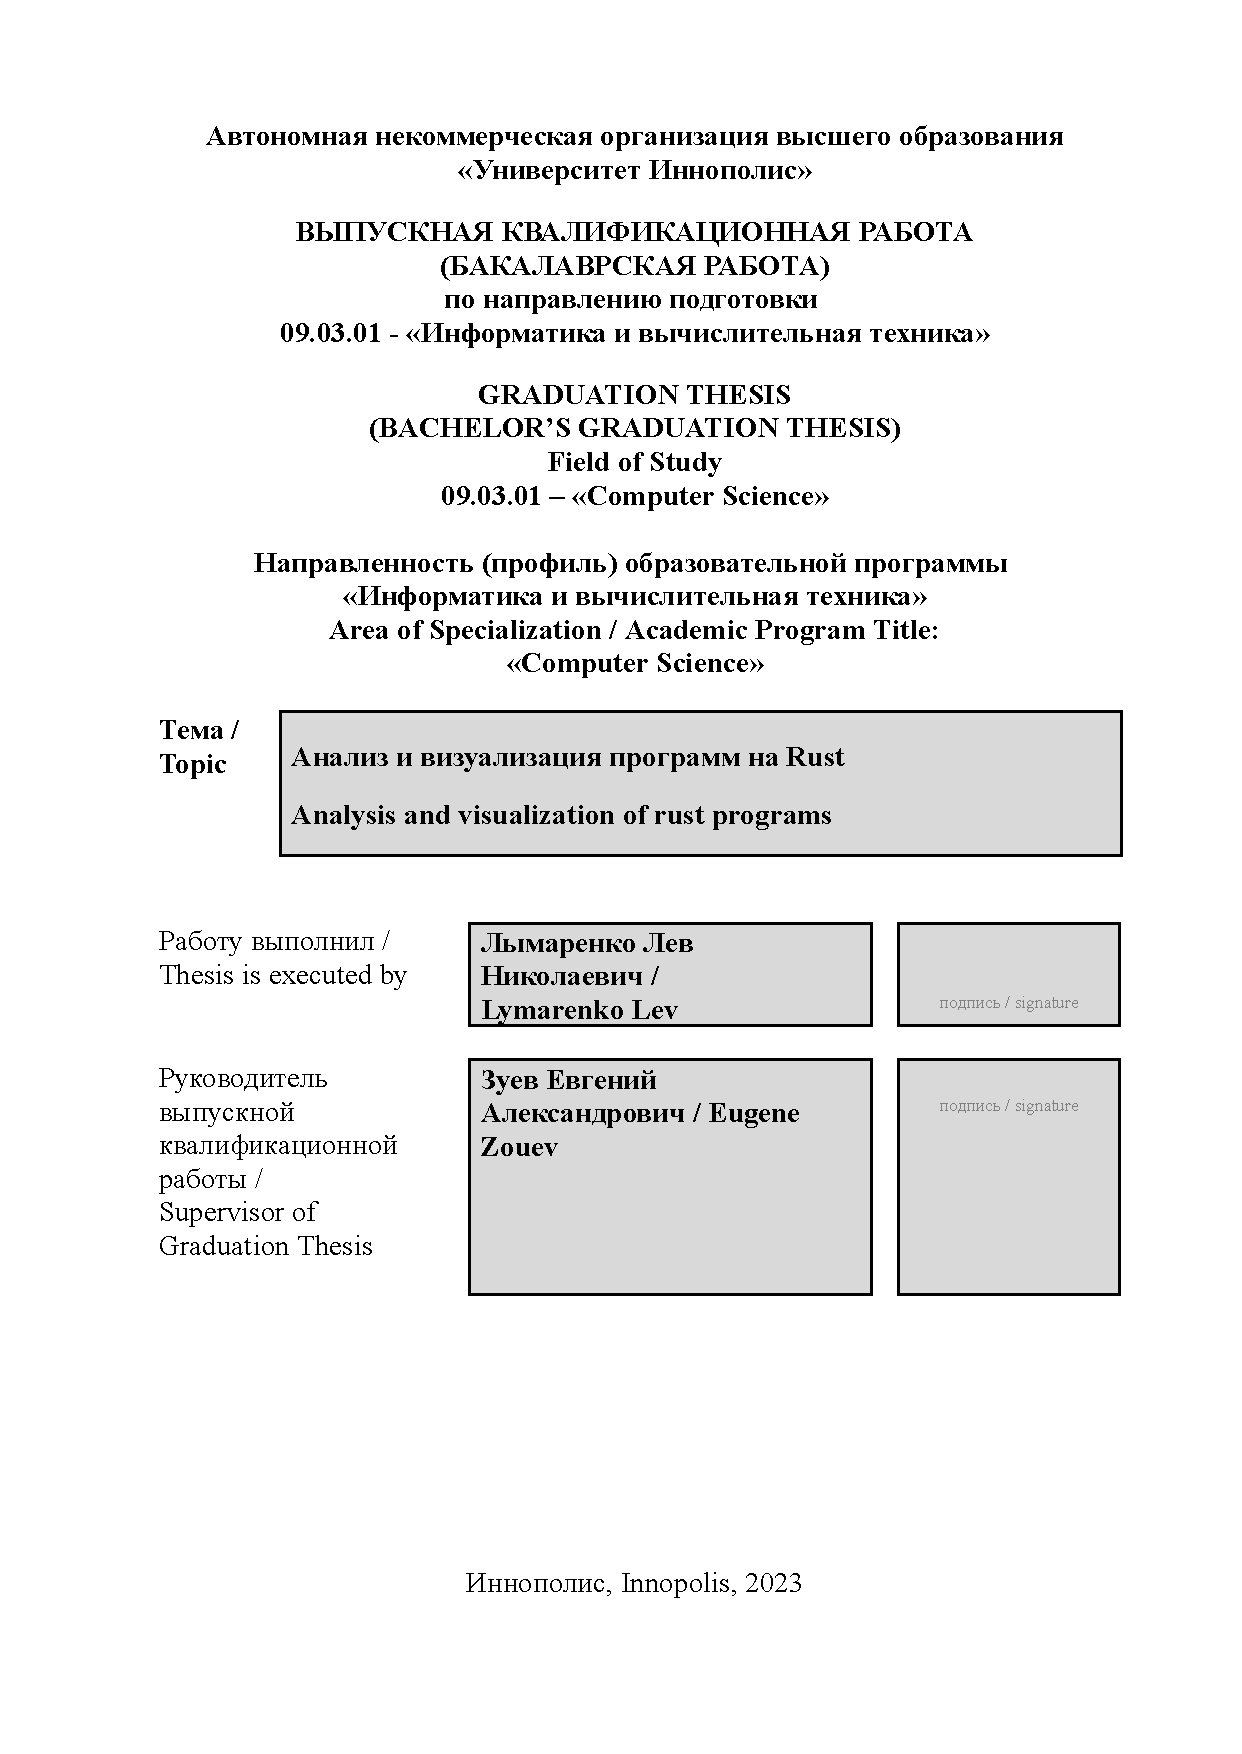
\includepdf[pages=-, offset=75 -75]{title.pdf}
\tableofcontents
\listoftables
\listoffigures


\newpage
\begin{abstract}
\par Static code analysis is popular among developers and IT specialists as it improves code comprehension and software architecture. Rust, an innovative and powerful language, can be challenging to understand due to its strong compile-time requirements. To address this, IDEs (Integrated Development Environments) with built-in static code analyzers have been developed. However, many existing tools are heavy and require additional dependencies, making IDEs inconvenient for code understanding and viewing.

In this thesis, we propose an alternative approach. Instead of an interactive text editor, we analyze Rust source code once and generate a ready-made HTML file with visualized code. This HTML file can be accessed through a regular browser without additional installations. We compare two methods of parsing Rust source code to create an Abstract Syntax Tree (AST), explain how we populate the AST with information about types, definitions, and cross-links between entities, and describe our process of generating a static HTML page with all the features found in a conventional IDE. Our application generates a static visualization of the project in the form of an HTML page called a report. This report can be easily shared without dependencies. It serves various purposes such as code review, onboarding new employees, or showcasing the project's results to customers.

The thesis concludes with an evaluation of the application's performance and limitations, as well as suggestions for future work. The HTML report generation application provides a valuable tool for Rust developers to navigate and understand code efficiently.

\end{abstract}

\setcounter{page}{7}
\chapter{Introduction}
\label{chap:intro}

\section{Background and Motivation}

Software development is a complex task that involves writing and maintaining large codebases. As projects grow in size and complexity, it becomes increasingly difficult for developers to understand the code and identify potential issues. One of the primary challenges that developers face is the need to comprehend programs quickly and accurately. This is particularly challenging when working with code that was written a long time ago by different people and lacks proper documentation.

To address this challenge, developers have turned to various tools and programs that can help them comprehend and write code more conveniently. These tools are designed to make the development process more efficient by providing developers with the information they need to navigate the project effectively.

One of the most popular and useful approaches to this problem is text program visualization. This approach is used in many IDEs, code viewers, and documentation generators and is characterized by several key features. One of the most important features of text program visualization is syntax highlighting. This feature involves highlighting different parts of the code in different colors to make it easier for developers to identify keywords, functions, and other important elements of the code. This makes it easier to scan through the code and identify potential issues quickly.

Another important feature of text program visualization is the use of cross-entity links. These links allow developers to move easily between different parts of the project, such as functions, definitions, and other elements. This makes it easier for developers to navigate the codebase and understand the relationships between different parts of the code.

In addition to these features, text program visualization tools also provide information about the declaration and usage of variables and other elements of the code. This information can be critical for understanding how the code works and identifying potential issues that may arise.

Overall, text program visualization has become an essential tool for software developers. It provides a powerful and efficient way to comprehend and write code more conveniently. By leveraging the features of text program visualization, developers can work more efficiently and effectively, reducing the time and effort required to develop and maintain complex projects.

\section{Task description}

The aim of this thesis is to develop an autonomous tool that will analyze modern and popular Rust programming language and convert it into a portable \textit{HTML} format, which can be easily opened with any popular web browser. This tool is intended to provide an extensive code visualization functionality to the users, which will help them to quickly understand and comprehend the Rust code.

The task involves developing a software tool that will analyze the Rust code, extract the relevant information, and present it in a visually appealing and easy-to-understand format. The tool should be able to handle large and complex codebases, which may have been written by different people, and may not have any documentation.

To achieve this goal, the tool will leverage the popular and useful features of existing solutions in the field of Rust code text visualization, such as syntax highlighting, cross-entity links, and displaying information about declaration and usage. However, unlike existing solutions, our tool will focus on providing cross-platform portability by generating a report in the form of a single HTML file.

The tool will be mainly used by developers who need to quickly understand the code, such as a supervisor of an intern who needs to review the code, a person who just joined a large company and needs to understand the project as quickly as possible, or a customer who wants to see the result of the project by looking at the internal code implementation.

The development of this tool involves several stages, including research on Rust programming language, analyzing the existing solutions for Rust code text visualization, designing the architecture of the tool, implementing the tool, and testing it for various use cases. The final outcome of this thesis is fully functional tool that can be used by developers to understand and comprehend the Rust code in a more convenient and efficient way.

\section{Applicability}

The application developed in this thesis will have numerous applications in the field of Rust development. First and foremost, it will serve as a valuable tool for developers who need to understand the structure and workings of a Rust project. By providing a detailed and navigable HTML report, the application will make it easier for developers to explore the codebase and identify potential issues.

The application will also be useful for project managers and other stakeholders who need to review Rust projects. By providing a clear and concise overview of the codebase, the report will allow these individuals to assess the project's progress and identify any areas that require further attention.

Finally, the application will be useful for researchers and educators who need to study the Rust programming language. By providing a detailed and navigable HTML report of a Rust project, the application will make it easier for these individuals to explore the language and understand its various elements. Additionally, the application can be used as a teaching tool to introduce students to Rust programming and provide them with hands-on experience exploring a real-world project.


\chapter{Literature Review}
\label{chap:lr}

This chapter gives information about the concepts and techniques that we will use.
In addition, we provide a summary of the most common tools for visualizing Rust source code.
Section \ref{sec:vis} describes the notion of visualization, its examples, and its types.
Section \ref{sec:html} gives a brief description of the HTML language that we will use to build the final report.
In section \ref{sec:rust} we talk about Rust, and why we decided to choose this language.
Section \ref{sec:anal} discusses how to perform static analysis of Rust code.
Section \ref{sec:sol} presents the most popular existing solutions for visualization, describes and evaluates them.
We make a conclusion about visualization and current solutions, describing their advantages and disadvantages in section \ref{sec:conc}.


% Software development is a rather complicated and not straightforward task. 
% In big projects, there are thousands of lines of code and hundreds of files in which a programmer should be able to understand what is happening to develop or maintain the project. 
% To fulfill this need, program visualization was introduced.

\section{Source code visualization}
\label{sec:vis}
In big projects, there are thousands of lines of code and hundreds of files in which a programmer should be able to understand what is happening to develop or maintain the project. 
To fulfill this need, program visualization was introduced.

Program visualization is a mapping from programs to graphical representations \cite{247643}. Architecture diagrams, dependency graphs, and, code visualization help to see the overall picture presented in the program. 
For example, \cite{cvsscan} introduces visualization of code evolution. It is an integrated environment to track code changes, the contributors' roles, and the history of a project using line-oriented displays.
ViLLE \cite{ville} is another example of program visualization. It has several features, for example, code editing, tracing execution, code line explanation, and language-independency. Also, ViLLE team conducted research and concluded that code visualization improves students' learning regardless of their programming skills.

There are several types of program visualization. The most popular one is text visualization which is offered by many IDE.
It consists of all possible options for modifying the source code, for example, adding hints in the text, coloring keywords or other tokens, accentuating logical blocks, icons, color highlights, and code navigation \cite{2018visual}. 
Figure \ref{fig:hl_example_1} shows an example of visualizing a source code. Here end user can see, for example, highlighted syntax, and additional information about the types of variables and functions documentation.

Source code visualization is quite popular nowadays since it provides detailed information about the project. In addition, it is a useful tool for newcomers to overcome the barrier of a huge amount of information available at the start \cite{5336433}. 

To sum up, program visualization is a popular and useful tool for developing and maintaining a projects. 
There are several types and examples of visualization. Text visualization is widely used by developers today because it offers an intuitive environment for navigating and explaining code.

\begin{figure}[hbt]
\centering
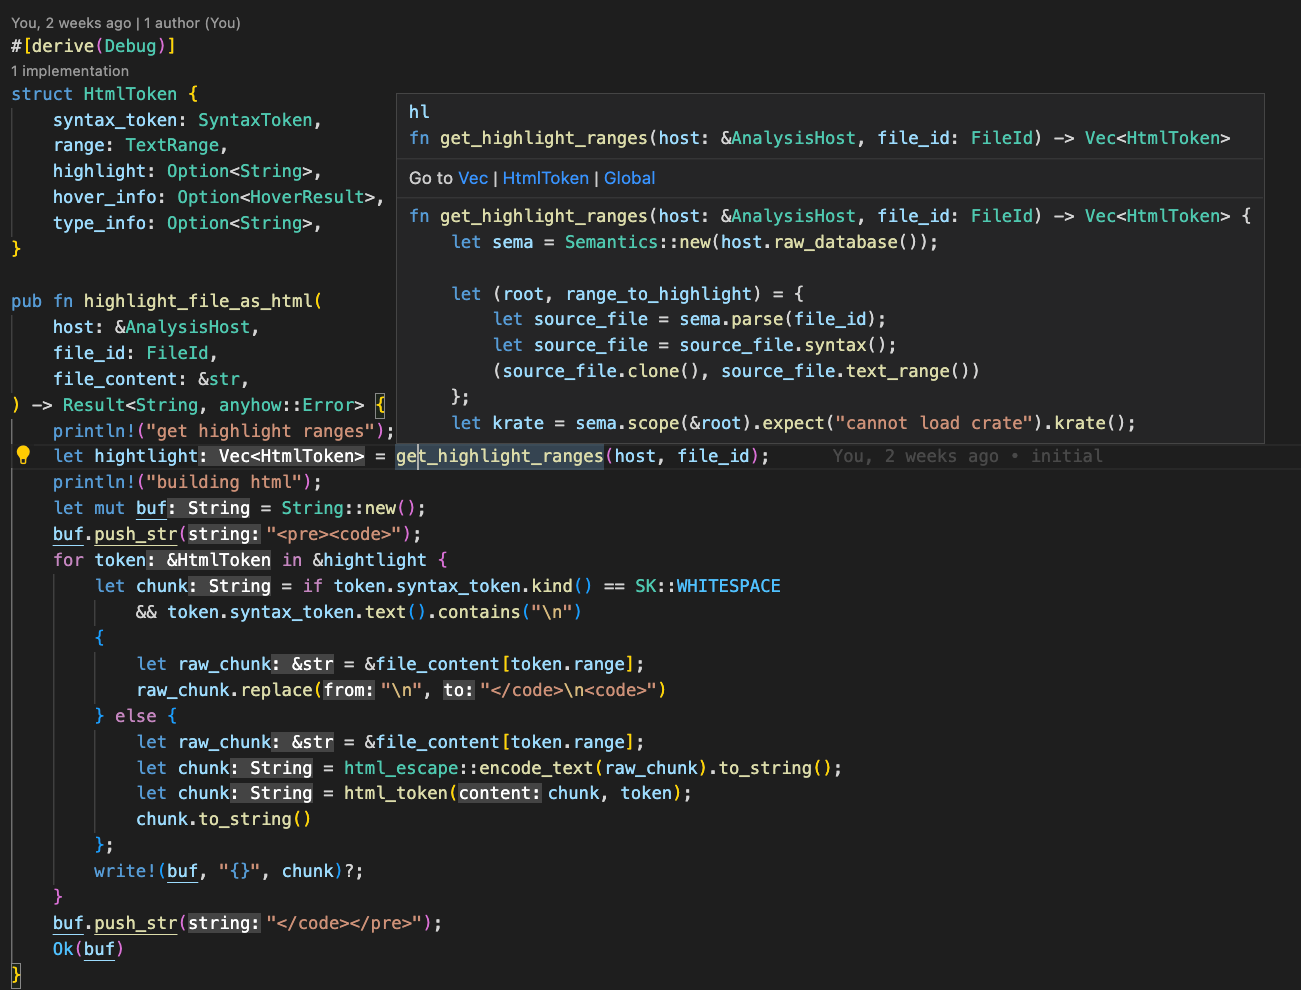
\includegraphics[width=15cm]{figs/hl_example_2.png}
\caption{Source code visualization example}
\label{fig:hl_example_1}
\end{figure}



\section{Visualization via HTML}
\label{sec:html}

HTML is the markup language for creating Web pages. It can be used for text visualization. It has a lot of built-in features that will help us to implement all the visualization features that we want. The main advantage of HTML over other visualization methods is that it is popular and widely used. Every modern browser can show an HTML page without additional dependencies and internet access.
Visualization via HTML is quite popular nowadays. 
GitHub \cite{github} is web storage of source code, that supports HTML highlighting for over 1000 languages.
Another example is \textit{Online Python Tutor}. It is a web-based program visualization tool for Python \cite{python}. Using that tool users can write programs in the browser with a visualization of each execution step.

% \section{Program static analysis}
% \label{sec:2anal}


% TODO: too small
% how it's related to visualization


\section{The Rust language}
\label{sec:rust}
Rust is a new programming language for developing reliable and efficient systems \cite{rust-official}.
Currently, Rust is gaining popularity, and some companies prefer it rather than C++ \cite{top-lang}. 

Rust provides a wide range of high-level features, such as static typing, thread, and memory safe together with low-level features such as full memory control.
Rust has 48 keywords (31 currently used keywords and 17 reserved for future use). For example, in the C++ language that is most similar to Rust in terms of application area, there are 95 keywords which are almost twice as many. 
There are no header files in Rust and a big project can be divided into encapsulated crates and modules that provide convenient and readable architecture. 
Rust developers were able to make a memory-safe system without a garbage collector using compiler-checked abstractions. A strong ownership system ensures programmers that, for example, there will not be a memory leak, uninitialized memory access or data-race problem \cite{reed2015patina}.
Another advantage of choosing Rust as the language for this study is that although it is a complex syntactic language, it provides an open API for static code analysis, so the development of a code visualizer will not go into the task of developing its compiler.
But at the same time, Rust also has drawbacks: it has a rather complex syntax for beginners and it lacks a lot of user libraries, due to its novelty.

To sum up, we decided to choose Rust language because it is modern, relatively popular, and powerful. Using that language big and complicated projects can be built, so code visualization would be helpful in this situation.

\section{Rust source code analysis}
\label{sec:anal}
Static analysis is strongly connected to source code visualization. In order to visualize the program code, we should represent the code in a more informative data structure. For this purpose, source code parsing, the first step of every static analysis approach, is used. This is a process of representing a set of characters into a more abstract and useful data structure, for example, an Abstract Syntax Tree (AST). 

Static program analysis is a way to analyze a program without running it. It takes source code and produces a report, for example, a bug report in software \cite{anal}. MirChecker \cite{mirchecker} is an example of applying static analysis of MIR (mid-level intermediate representation provided by Rust compiler) to automatically find bugs in Rust programs. 

The programming language syntax is a set of language rules. It defines how to write valid programs and what is the structure of these programs. As was mentioned before, Rust has a fairly rich syntax that allows users to use complex constructs such as generic, macros, error propagation, lambda functions, a lifetime of variables, and many others. 
Because of this, for beginners, Rust may seem complicated and even verbose. However, in this case, highlighting tokens could be helpful for newcomers.

\textit{Syn} is a Rust crate that is used to parse a stream of tokens into a Rust syntax tree and its main purpose is to write procedural macros in Rust \cite{crates-syn}. 
\textit{Rust-analyzer} is a set of crates for semantic analysis of Rust code. It uses MIR analysis internally and provides API to analyze source code and obtain meta information about tokens, such as definition place, references, and inferred type information \cite{crates-rust-analyzer}. Later, in the methodology section, we will discuss how those crates will help us build the parsing module of our application.

% Nevertheless, complicated syntax is problem for parsing and static analyzing and Rust solves this problem by introducing high-level intermediate mid-level intermediate representation (MIR) of source code. This presentation can be obtained from the compiler and represented as modified source code with expanded macros, explicit types and simplified constructions. 
Summing up, static analysis is closely related to text visualization. Rust syntax is quite complicated, however, Rust offers clear API to perform source code analysis.

\section{Existing solutions}
\label{sec:sol}

In this section, we will discuss existing solutions for Rust code visualization, and understand what their disadvantages are.

\begin{enumerate}[label=\arabic*)]
    \item \textbf{Visual Studio Code extension} - Rust has its own extension for VSCode IDE. The extension is built on top of the \textit{rust-analyzer} \cite{crates-rust-analyzer} library. It provides some of the required functionality via the Language Server Protocol, however, it is geared toward writing code, and, therefore, requires installation of VSCode, its dependencies, and the extension itself. In addition, there is no portable output of the project, so this solution is powerful, but not appropriate for our case.

    \item \textbf{Rustdoc} - is a tool to generate HTML documentation for Rust source code \cite{rustdoc}, for example, additional comments for modules, function signatures, and trait implementations. It also provides a feature to browse source code. However, it lacks many useful features, for example, identifier information, jumps to references, and type of variables. Also, it shows \textit{.rs} files only, which is logical for documentation purposes, but inconvenient for a full understanding of the project.

    \item \textbf{github.com} - Internet hosting site for version control system \cite{github}. Used to store source code of projects. It provides basic highlighting and static code analysis such as showing definitions and references. However it requires loading every source code page over the internet, it doesn't have a project tree and it has the least number of visualization features of all the solutions presented since visualization is a secondary feature of GitHub.
\end{enumerate}

% github.com - only highlitgh

% vscode + rust-analyzer -- very powerful, but havy, doesn't produce static file

% rustdoc - similar to what we want, but lack of some usefull features
% novelty
% to the best of our knowledge, there is no existing solution 
% we offer 

\section{Conclusion}
\label{sec:conc}

In conclusion, among the many types of visualization, we decided to choose text visualization as the most popular and widely used. 
There are solutions in the field of Rust code text visualization, however, they all lack usability or portability, or they require the installation of many dependencies since they indented to write and change the source code.
Our solution is to use a portable and cross-platform visualization format such as HTML and use all the known useful features to explore the program text conveniently.

\newpage


\chapter{Methodology}
\label{chap:met}

This section provides a comprehensive overview of the software requirements and methods employed in this thesis. Section \ref{meth:req} outlines the essential requirements that were established at the outset of the study, emphasizing that their fulfillment is essential for the successful completion of the thesis. Additionally, we discuss the inclusion of supplementary requirements, which are not mandatory but offer potential for the integration of additional features. In Section \ref{meth:design}, we delve into the design choices made for the application, elaborating on the underlying decisions that influenced its development. Section \ref{meth:modules} provides a concise overview of the various modules comprising the application.

\section{Software Requirements}
\label{meth:req}
The goal of this thesis is to create an application that will allow developers to quickly and easily understand and navigate Rust source code. The purpose of the application is to provide developers with a lightweight, HTML-based report of a project that contains all of the essential features and information they need to efficiently and effectively develop software using Rust programming language. The report should be designed to be both informative and engaging, with clear, concise information about the project and its components. The report should also be easy to use, with intuitive navigation features that make it easy for developers to access and understand the information it provides. By creating a report that combines the best features of IDE's, this application will help to improve development process and make it easier and faster to work with Rust projects.


% TODO: MUST/DONE/ ??
We have opted to partition the project requirements into two distinct tables, namely "Obligatory" and "Additional" requirements. Table \ref{table:must_req} delineates the set of requirements that are deemed mandatory for the successful completion of the project:

% \begin{longtable}{c|c}
% \caption[Requirements for the project]{Project requirements} \label{table:req} \\
% \hline
% Feature & Description  \\
% \hline
% \endhead
% \hline
%  Project tree & The report should provide a comprehensive project tree that displays the structure of the project, including all of the files and folders within the project. This tree view should allow developers to easily navigate the project and understand its structure \\
%  \hline
% \end{longtable}

\begin{longtable}{|p{1.5in}|p{4in}|}
\caption[Obligatory requirements]{Obligatory requirements}\label{table:must_req}\hline
Feature name & Description\\\hline
1. The report &
The application should scan the project directory and generate a comprehensive HTML file, referred to as the "report". The report should provide an overview of the project, including a tree view of the project folders and files.\\\hline

2. Portability & The report must be a single file that works on all popular web browsers. It should be optimized for web use with fast loading times and responsive design for various screen sizes. \\\hline

3. Related files & The application should have the ability to ignore certain files and directories, such as binary files, build directories, static images which are not relevant to the development process. This will ensure that the report is clean and easy to read, only displaying relevant information. \\\hline

4. File content & By clicking on a filename in the project tree, the report should display the content of that file. This will allow developers to quickly access the source code and view it in a clean, formatted manner. \\\hline

5. Highlight & The content of the report should be highlighted, easy-to-read manner, with the lines in the file number for reference. This will make it easier for developers to navigate the code and understand its structure. \\\hline

6. Hover information & When hovering the cursor over a token, the report should provide additional information about it, including the signature of the function or the type of variable, the path of its declaration, and any associated doc strings. This will make it easier for developers to understand the code and its functionality. \\\hline

7. Navigation menu & By clicking on a token, the report should open a navigation menu that displays information about the definition and references of the token. The navigation menu should have two tabs: Definition and References. The Definition tab should be open by default and contain links to the file and line number of the struct, function, or module definition. The References tab should contain links to the file and line number of all struct, function, or module usage, making it easy for developers to find and understand references to the token. \\\hline

8. Return to original location & The report must allow developers to easily return to the place where they began a navigation jump. This feature will enable developers to quickly move between different parts of a project without losing their place or becoming disoriented. \\\hline

9. Hiding block expressions & The application must provide the ability to hide and show large blocks of code, such as functions, modules, or other block expressions \cite{rust-book-code-blocks}, for improved code readability. This feature will enable developers to focus on specific areas of code without being overwhelmed by the complexity of the entire project.\\\hline 

10. User-friendly interface & The report should be intuitive and user-friendly, with a clear structure, and be similar to modern IDEs. This will improve the overall development process and make it easier for developers to work with Rust programs.\\\hline

\end{longtable}

Table \ref{table:could_req} describes requirements that could be done or could be considered as direction for further work.

\begin{longtable}{|p{1.5in}|p{4in}|}
\caption[Additional requirements]{Additional requirements}\label{table:could_req}\\\hline
Feature name & Description\\\hline
1. Customizable style themes & The report should provide developers with the ability to customize the style theme dynamically using pre-set style themes. This will help to improve the overall usability and accessibility. \\\hline

2. Project search & The report must include a robust code search feature that allows developers to quickly search for specific symbols within the whole scanned project.\\\hline

3. Errors & The application must generate a report even if the project contains syntax errors or warnings. The report should clearly indicate the location and type of errors or warnings, and provide suggestions or solutions to fix them. \\\hline

\end{longtable}



\section{Design}
\label{meth:design}
\begin{figure}[ht]
\centering
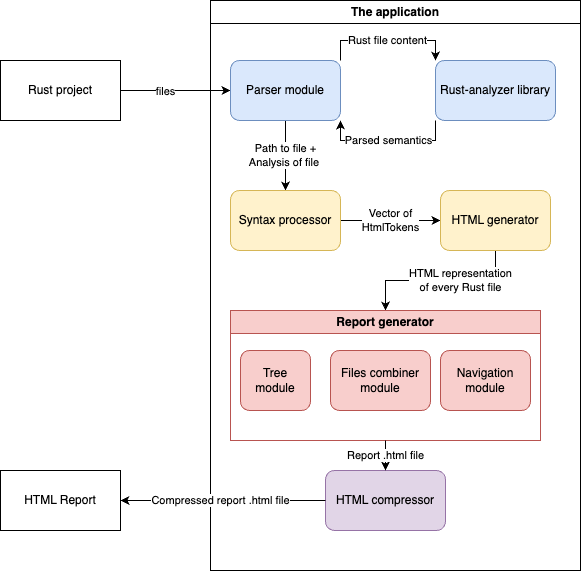
\includegraphics[width=15cm]{figs/thesis_flow3.png}
\caption{Architecture of the HTML generation process}
\label{fig:flow}
\end{figure}


This section describes the architecture of the HTML report generation application for Rust projects. It provides a detailed explanation of the steps taken to develop the application, including the technologies used, the algorithms designed, and the challenges faced during the development process.

The design chapter of the HTML report generation application aims to outline the various modules and their interconnectedness that facilitate the generation of a single HTML report file. The process of software development is a complex task that requires a deep understanding of the codebase, especially when working with code written by different people and lacking in documentation. To address this problem, developers have increasingly turned to special programs and tools that make comprehending and writing code more convenient. Among these approaches, text program visualization has emerged as the most popular and useful method, employed in most Integrated Development Environments (IDE), code viewers, and documentation generators.

The HTML report generation application adopts a modular approach, consisting of several interconnected modules that work together to produce a single HTML report file. The flow of data through the application starts with the Parser module, which scans the Rust project directory and receives all the files. Each file is then sent to the Rust-analyzer library, which generates a semantics object for every source file and an analysis object for the entire project. The Parser module builds analysis of file, which is passed to the Syntax processor. The Syntax processor evaluates analysis of file, and generates a vector of HTML tokens for each file. These vectors are then forwarded to the HTML generator, which combines them into an HTML representation of one file. The resulting file is then sent to the Report generator.

The Report generator comprises three interconnected modules: the Tree module, the Files combiner module, and the Navigation module. The Tree module generates a tree structure of the Rust project, which acts as an overview of the entire codebase. The Files combiner module combines all the HTML representations of individual files generated by the HTML generator into a single file. The Navigation module provides additional functionality to the report, such as code jumping to functions and definitions and displaying information about variables when the user's cursor hovers over them. Once all the modules have performed their tasks, the report is sent to the HTML compressor, which compresses the HTML to decrease the size of the final report.

To implement this design, which can be viewed as a diagram in Fig.\ref{fig:flow}, the application was developed using the Rust programming language and several external libraries, including Rust-analyzer \cite{crates-rust-analyzer}, Syn \cite{crates-syn}, Tera \cite{tera-official} and minify \cite{minify-github}. The modular design of the application allows for easy customization and extension, ensuring that the application remains flexible and adaptable to meet the evolving needs of Rust developers. The application also features a user-friendly interface that allows users to specify the location of the Rust project directory, output format, and compression level for the HTML report. The end result is an efficient and intuitive application that streamlines the process of code comprehension and makes Rust development more convenient and productive.

% To improve the readability of the HTML report, we added CSS styling. We designed the CSS to make the code more visually appealing and easier to read by using color-coding, font styles, and other design elements.

% Finally, we compiled the resulting binary file for Linux x86 to ensure that the project is easily accessible to all developers. The launch of the binary file can be customized via command-line arguments, allowing users to adjust the application's behavior as needed.

% Overall, our goal in designing the application was to provide developers with a powerful tool that is both intuitive and user-friendly. By combining the strengths of Rust and rust-analyzer with modern web design principles, we believe that our application will provide developers with a new level of efficiency and ease of use when working with Rust code.


\section{Overview of Modules}
\label{meth:modules}
This section provides a comprehensive description of the modules that have been developed as part of the HTML report generation tool for Rust programming language. Specifically, it includes a detailed description of the parser \ref{chap:modules:parser}, Syntax processor \ref{chap:modules:processor}, HTML generator \ref{chap:modules:generator}, report generator \ref{chap:modules:report_generator}, and compressor modules.

\subsection{Parser Module}
\label{chap:modules:parser}

These sections describe possible approaches to code parsing, their compatibility with the project, and the challenges faced during the implementation of the parser module.

Parsing code accurately is a crucial task in the domain of static analysis. Several approaches exist for performing this task, with varying degrees of complexity and effectiveness.

% There are several possible solutions to the challenge of code parsing, each with its own benefits and drawbacks. One option is to use the Rust compiler, which is open-source and available on GitHub \cite{rust-github}. The primary advantage of this solution is the closeness of the parsing results to the current state of the project, since the same code is used for both project compilation and parsing. However, while the Rust compiler's output can be highly accurate, the codebase is quite extensive and the API for obtaining static information about the code is not very user-friendly.

% Rust-analyzer is a compiler frontend library specifically designed for Rust. It provides a convenient and well-designed API for extracting information about the codebase's abstract syntax tree (AST). The rust-analyzer library is optimized for parsing large codebases, and it does not involve compiling the code, making it a more efficient choice for our project. Additionally, the library is modular and easy to use, making it a good fit for our needs. By using rust-analyzer, we were able to extract detailed information about the codebase's syntax, including information about tokens, types, and range, as well as information about definitions and references. This information is used to create an array of structs for generating the HTML report.


%%%%%

One approach involves building a custom parsing solution from scratch, which essentially involves implementing the initial stages of a compiler, including lexical analysis, syntactic parsing, and semantic analysis. While this approach may be necessary in some situations where a suitable solution is required, it can be a time-consuming and effort-intensive process, particularly in complex projects. Thus, it turned out to be unsuitable for the present project.

Another approach involves using existing compiler tools, which are open-source and available on GitHub \cite{rust-github}, to extract the necessary information. As the parsing of code is the first step in the compilation process, the compiler already possesses this information. Extracted compilation information is exactly what is required for our Parser module. The primary advantage of this solution is the closeness of the parsing results to the current state of the target project since the same code is used for both project compilation and parsing. Initially, this approach was chosen for the project. However, several difficulties were encountered during its implementation. For instance, the Rust compiler is a large and unwieldy project, making it challenging to extract intermediate compilation results from it. Moreover, it proved problematic to obtain cross-entity relations necessary for comprehending where functions and variables were declared. Additionally, this approach is unable to produce information in cases where the code was written with compile errors. Consequently, this approach was abandoned in favor of a different solution.

The third approach, which was ultimately adopted in this project, involves utilizing a third-party solution to analyze Rust source code. In particular, the Rust-analyzer \cite{crates-rust-analyzer} project was chosen for its open-source implementation of the Language Server Protocol \cite{lsp} for the Visual Studio Code IDE. Additionally, the Rust-analyzer provides a Rust library API that allows users to analyze Rust codebases comprehensively, including parsed AST (Abstract Syntax Tree), cross-entity relations, and searching for references, among other features related to IDE. This approach aligns well with the present project's requirements and provides all the necessary information to implement all visualization features. However, usage of Rust-analyzer tool also has several drawbacks, such as long loading times due to indexing all dependencies and a lack of API documentation. Nevertheless, the utilization of the Rust-analyzer for the parsing module is the most optimal solution available. By using Rust-analyzer, we were able to extract detailed information about the codebase's syntax, including information about tokens, types, and ranges, as well as information about definitions and references. This data are passed to the Syntax processor module \ref{chap:modules:processor}.

Overall, the Rust-analyzer library was the best choice for our project, as it provides user-friendly API and was designed specifically for parsing Rust code. Its modular and efficient design allowed us to extract the necessary information from the codebase quickly and accurately, and it ultimately helped us to create a powerful and efficient tool for navigating and understanding Rust code.

\subsection{Syntax processor}
\label{chap:modules:processor}
The primary objective of the Syntax processor module is to extract relevant information from Rust-analyzer about one source file and generate a vector of HtmlToken objects. These tokens encapsulate data pertaining to syntax highlighting, hover functionality, and navigation information. It is crucial to emphasize that the processor does not directly render HTML content; rather, it focuses on processing the output of Rust-analyzer and aggregating it into a convenient data structure for next modules.

A more comprehensive elucidation of this module will be expounded upon in Section \ref{chap:impl:processor}.


\subsection{HTML generator}
\label{chap:modules:generator}

The HTML generator module assumes responsibility for the rendering HTML content for source file. Its primary function entails transforming the conveniently structured representation of a file, as provided by the parser module, into corresponding HTML content for the given file. The rendering process occurs in two distinct steps, each serving a specific purpose.

Firstly, the module generates a vector of Line structures. Each Line structure contains essential information such as the line number, the rendered HTML content of the line, and collapse information. The inclusion of collapse information serves the purpose of fulfilling the requirement outlined in Table \ref{table:must_req}, which pertains to the implementation of hiding block expressions.

Secondly, the generated vector of Line structures is passed to the Tera template engine \cite{tera-official}, which serves as a Rust-based alternative to the widely used Jinja library \cite{jinja-official}. Tera template handles the appropriate placement of line contents and ensures the correct line-collapsing behavior in accordance with the specified requirements.

A more detailed examination of this module will be provided in Section \ref{chap:impl:generator}.

\subsection{Report generator}
\label{chap:modules:report_generator}

The report generator module serves as a central entity responsible for combining and integrating diverse elements, including file content generated by the HTML generator module, tree content derived from the tree module, navigation content, and static CSS files. Similar to the HTML generator module, the report generator leverages the capabilities of Tera templates to facilitate the generation of the final output HTML file.

Further elaboration on the implementation details of the report generator module can be found in Section \ref{chap:impl:report_generator}


\subsection{Compressor}
\label{chap:modules:compressor}
In comparison to other modules, the compressor module serves as a compact component integrated with the Minify Rust crate \cite{minify-github}. Its primary function is to perform a straightforward yet crucial task, which involves diminishing the size of the output file while preserving its content. This is achieved by eliminating redundant spaces and tabs, and shortening JavaScript and CSS segments, among other optimizations.

Regarding quantitative measurements, the incorporation of the compressor module has resulted in a substantial reduction of approximately six times in the number of lines within the final report file, accompanied by a 25\% decrease in file size, as quantified in bytes. This step holds significance in relation to the Portability feature outlined in the requirements, as depicted in Table \ref{table:must_req}.

\section{Conclusion}
In this chapter, we provided functional requirements and an overview of the various modules developed as part of the HTML report generation tool for the Rust programming language. These modules include the parser, Syntax processor, HTML generator, report generator, and compressor.

The parser module plays a critical role in accurately parsing the code and extracting essential information for static analysis. We explored different approaches to code parsing, including building a custom solution, utilizing existing compiler tools, and leveraging third-party solutions. After careful consideration, we selected the Rust-analyzer as the most suitable option, as it offers a well-designed API and comprehensive analysis capabilities. The integration of the Rust-analyzer facilitated the extraction of detailed syntax information, such as tokens, types, and ranges, enabling the creation of a data structure that serves as input for the Syntax processor module.

The Syntax processor module focuses on processing the output of the Rust-analyzer and aggregating relevant information into HtmlToken objects. These objects encapsulate data related to syntax highlighting, hover functionality, and navigation, providing a convenient data structure for subsequent modules.

The HTML generator module transforms the structured representation of a source file, generated by the parser module, into corresponding HTML content. It involves generating Line structures and utilizing the Tera template engine for rendering HTML and implementing line-collapsing functionality.

The report generator module acts as a central entity that combines file content, tree content, navigation information, and static files to generate the final output HTML file. It employs Tera templates for the effective generation and integration of these elements.

Finally, the compressor module, integrated with the Minify Rust crate, plays a crucial role in reducing the size of the output file while preserving its content. By removing unnecessary spaces, and tabs, and shortening JavaScript and CSS segments, significantly reduces the number of lines and file size, enhancing the portability of the generated HTML report.

In conclusion, the design and implementation of these modules have contributed to the development of a powerful and efficient HTML read-only IDE for the Rust programming language. The careful selection of tools and the integration of optimization techniques have resulted in a tool that facilitates code comprehension, navigation, and analysis, ultimately enhancing the development workflow for Rust programmers.



\chapter{Implementation}
\label{chap:impl}

The implementation section of this thesis provides a detailed account of the code written to accomplish the project's objectives. This section is essential as it offers insights into the technical aspects of the implementation process and demonstrates how the different modules work together to achieve the desired functionality. The section covers four main modules: Parser \ref{chap:impl:parser}, Syntax Processor \ref{chap:impl:processor}, HTML Generator \ref{chap:impl:generator}, and Report Generation \ref{chap:impl:report_generator}. By providing a comprehensive overview of the implementation process and the functionalities of each module, this section allows readers to gain a deeper understanding of the technical aspects behind the project's execution.


\section{Parser}
\label{chap:impl:parser}
The parser module is responsible for the implementation of a straightforward logic consisting of four steps. These steps involve scanning the directory, filtering the files, passing the files to Rust-analyzer, and generating a convenient response for the subsequent module.

The scanning process involves a recursive traversal of the target directory to locate the \textbf{Cargo.toml} file to find the root path of a Rust project. While this step is relatively unremarkable, it serves as a necessary foundation for subsequent operations.

Filtering assumes significance as it aims to include not only the .rs Rust files but also various other files such as configuration files and templates. However, it is essential to exclude certain files, such as build outputs, temp files, and the GIT directory, to avoid an excessive number of irrelevant files. To address this, we have devised a solution utilizing predefined glob patterns that allow us to ignore specific files and directories, such as the \textbf{/target}, \textbf{/.git}, \textbf{.vscode} directories . Additionally, we take into consideration the presence of a \textbf{.gitignore} file within the target project, as it may already contain relevant information about files to be ignored.

Following the filtering stage, the obtained information is passed to Rust-analyzer. This tool performs indexing on all project files and dependencies, yielding an Analysis object that encapsulates the results. Subsequently, this analysis object is utilized within the Syntax processor.

\section{Syntax Processor}
\label{chap:impl:processor}

The syntax processor module is responsible for traversing the syntax tree provided by Rust-analyzer. Its main task is to generate HTML tokens based on each syntax token encountered. To better understand the HTML tokens, let us delve into the structure of an HTML token shown in Fig. \ref{fig:html_token}.

\begin{figure}[htb]
\begin{minted}
[frame=lines, framesep=2mm, fontsize=\small]
{rust}
pub struct HtmlToken {
    pub range: TextRange,
    pub content: String,
    pub is_new_line: bool,
    pub highlight: Option<String>,
    pub hover_info: Option<HoverResult>,
    pub navigation: Option<Navigation>,
}
\end{minted}
\caption{HTML Token structure. Output of syntax processor.}
\label{fig:html_token}
\end{figure}

The \texttt{HtmlToken} structure consists of several fields. In addition to the \texttt{range}, \texttt{content}, and \texttt{is\_new\_line} fields, which are essential for accurately displaying the token's content, there are three fields that are used for visualization purposes.

The \texttt{highlight} field provides information about the type of the token, such as whether it represents a function, macro, keyword, or string literal, among others.

The \texttt{hover\_info} field is responsible for displaying additional information when the user hovers over a token. This information could include details like function signatures or variable types.

The \texttt{navigation} field stores data related to navigation, including the location where a function, variable, or module is defined and the places where the token is referenced.

Due to limitations of the HTML generator, each HTML token can only occupy a single line. Therefore, if a token contains multiple newline characters, the syntax processor will split it into multiple HTML tokens, each having the \texttt{is\_new\_line} field set to true.

During the initial stages of this project, in the design process, we decided to store information about large code blocks during this syntax traversal to allow for the possibility of hiding them in the final HTML file. However, during the implementation phase, we discovered that Rust-analyzer already provides a public API related to folding ranges of code blocks. By utilizing this API, the syntax processor can also provide the HTML generator with the folding ranges, eliminating the need to calculating this information.


\section{HTML generator}
\label{chap:impl:generator}

The HTML generator can be considered as the main rendering component. Its primary purpose is to generate HTML code for a single source file. It receives a stream of HTML tokens from the syntax processor and performs the rendering of each token. The generated HTML content is then merged together, including line numbers and folding information.

Each HTML token is processed as a \texttt{<span>} HTML tag. The token's highlight information is encoded as class attributes of the \texttt{span} tag, the hover information is represented by an internal, invisible span tag by default, and the navigation information is encoded as a custom attribute \texttt{jump-data}.

Fig. \ref{fig:example_rendered_token} shows example of the rendered variable \texttt{files\_content}, which has the type \texttt{HashMap<String, String>}:

\begin{figure}[htb]
\begin{minted}
[frame=lines, framesep=2mm, fontsize=\footnotsize]
{text}
<span 
    class="hovertext variable declaration mutable"
    jump-data=...JSON ENCODED NAVIGATION DATA...
>files_content<span 
        class="hovertext-content"
        >HashMap&LTString, String></span></span>
\end{minted}
\caption{Example of rendered syntax token.}
\label{fig:example_rendered_token}
\end{figure}

After rendering each token, the generator merges the results together and splits them into lines. It then constructs a stream of \texttt{Line} structures. The \texttt{Line} structure is defined in Fig. \ref{fig:line}.

\begin{figure}[htb]
\begin{minted}
[frame=lines, framesep=2mm, fontsize=\small]
{rust}
struct Line {
    number: usize,
    html_content: String,
    fold: Option<FoldingRange>,
}
\end{minted}
\caption{Line structure. The output of HTML generator.}
\label{fig:line}
\end{figure}

The final step of the HTML generator involves combining the lines, line numbers, and folding information. This is accomplished by rendering an HTML template using the Tera engine \cite{tera-official}. Fig. \ref{fig:generator_template} shows the content of the generator's template. It can be observed that this code section employs a table layout to render line numbers and line content. Furthermore, the template utilizes all the fields of the Line structure, such as \texttt{line.fold}, \texttt{line.number}, and \texttt{line.html\_content}. To incorporate the folding (collapsing) logic and navigation functionality, JavaScript code is utilized. This code will be linked to the report during the final stage in the Report generator.

\begin{figure}[htb]
\begin{minted}
[frame=lines, framesep=2mm, fontsize=\footnotesize]
{html}
<table><tbody>

    <tr class="table-line" number="{{line.number}}">
        <td id="L{{line.number}}" class="prevent-select line-number">
            <a href="#L{{line.number}}">{{line.number}}</a>
        </td>
        
        <td
            id="LF{{line.number}}"
            class="prevent-select line-fold arrow arrow--right" 
            data-fold-start-line="{{line.fold.start_line}}"
            data-fold-end-line="{{line.fold.end_line}}">
        </td>
        
        <td></td>
        
        <td id="LC{{line.number}}" class="line-content"
        ><code><pre>{{line.html_content | safe}}</pre></code></td>
    </tr>

</tbody></table>
\end{minted}
\caption{Final HTML template of generator module.}
\label{fig:generator_template}
\end{figure}

\section{Report Generation}
\label{chap:impl:report_generator}

The report generation module plays a significant role in the overall system. Its purpose is to take the HTML-rendered files of the project and construct a final HTML report file. However, the resulting file should not only contain the content of the project files but also include additional information.

\subsection*{Tree Module}
To fulfill the requirement of including a project tree in the final report, as indicated in the features table \ref{table:must_req}, the report generator employs a tree module. This module receives the paths of the project files and generates an HTML representation of the project tree using the HTML \texttt{<input>} tag with different type attributes. Each file in the project tree is assigned the type \texttt{"radio"} to ensure that only one file can be displayed at a given time. This is achieved through radio buttons, which allow the user to select only one option from a limited number of files. On the other hand, directories in the project tree can have any number of open options, so they are assigned the type \texttt{"checkbox"}. Checkbox buttons enable the user to select zero, one, or multiple directories from a limited set.

\subsection*{Files Combiner}
Once the project tree has been constructed, the generator proceeds to merge all the files together and place them at the bottom of the report. These files are assigned an invisible class tag. During runtime, if the user clicks on a filename in the project tree, the navigation module locates the corresponding file content and displays it in the main code section.

\subsection*{Navigation}
\label{chap:impl:navigation}
The navigation module is the final sub-module of the report generator. It reads static files, such as CSS and JavaScript, and combines them into the final result. The JavaScript content is particularly crucial for achieving the desired functionality. It encompasses numerous tasks, such as handling user interactions with the project tree, dynamically changing the displayed file content, opening and closing the navigation menu, navigating to different files and lines, highlighting selected lines, preserving a history of jumps, and folding code blocks.

In addition to the JavaScript content related to navigation, the report generator also includes CSS content, which is essential for achieving an aesthetically pleasing and user-friendly layout for the IDE. The CSS styles govern various aspects, including text formatting, hover effects, code highlighting, and more. It also takes responsibility for ensuring the correct display of the project tree, wherein closed directories should hide their internal content.

We won't delve into the intricate details of CSS and JavaScript implementation in this thesis, as it requires in-depth knowledge of those fields. However, the source code can always be found in the project's GitHub repository \cite{sevenzing_2023_8017323} for a more comprehensive exploration of this section.

\subsubsection*{Final Merge}
Similar to the HTML generator, the report generator utilizes Tera templates to render the four components (tree, files, CSS, and JavaScript) into the final result. The Tera templates enable the seamless merging of these pieces to produce a comprehensive HTML report.

\newpage
\section{Conclusion}

In this implementation section, we discussed the details of how the code was written to achieve the objectives of the project. We described the four main modules: Parser, Syntax Processor, HTML Generator, and Report Generation, along with their respective functionalities. Fig. \ref{fig:pseudo_code} contains pseudo code and summarizes the data flow of the project, illustrating how the different modules work together to achieve the desired functionality.


\begin{figure}[htb]
\begin{minted}
[
frame=lines,
framesep=2mm,
baselinestretch=1.1,
fontsize=\footnotesize,
linenos
]
{python}
function run(root: Path) {
    parser = Parser::new(root)
    (files, analysis) = parser.scan_and_get_analysis()
    processor = SyntaxProcessor::new(analysis)
    html_tokens_map = {
        path: processor.process_file(path)
        for path in files
    }
    generator = HtmlGenerator::new()
    files_content_map = {
        path: generator.generate(html_tokens)
        for (path, html_tokens) in html_tokens_map
    }
    report_generator = ReportGenerator::new()
    output = report_generator.generate(
        files_content_map
    )
    compressed_output = compress_html(output)
    write_output(compressed_output)
}
\end{minted}
\caption{Pseudo code that describes data flow of the project.}
\label{fig:pseudo_code}
\end{figure}


The Parser module (lines 2-3) is responsible for scanning the project directory, filtering files, invoking Rust-analyzer for analysis, and preparing the data for further processing. It ensures that only relevant files are considered while excluding irrelevant ones.

The Syntax Processor module (lines 4-8) traverses the syntax tree provided by Rust-analyzer and generates HTML tokens for each encountered syntax token. These tokens contain essential information about the code elements such as their range, content, highlighting, hover information, and navigation details.

The HTML Generator module (lines 10-13) takes the HTML tokens from the Syntax Processor and performs rendering, including line numbers and folding information. It utilizes a template engine to combine the rendered tokens into a cohesive HTML report for each source file.

The Report Generation module (lines 15-17) constructs the final HTML report file by incorporating the HTML-rendered files, project tree, navigation functionality, and CSS styles. It utilizes various sub-modules such as the tree module for representing the project tree, the files combiner for merging project files, and the navigation module for handling user interactions and enabling navigation within the report.

\chapter{Conclusion}
\label{chap:conclusion}

In this thesis, we have successfully developed an HTML read-only Integrated Development Environment (IDE) for the Rust programming language \cite{sevenzing_2023_8017323}. The aim of the tool was to provide a comprehensive code visualization functionality to aid developers in quickly understanding and comprehending Rust code. We have achieved this goal by leveraging the popular features of existing solutions in the field of Rust code text visualization, such as syntax highlighting, cross-entity links, and displaying information about declaration and usage. However, unlike existing solutions, our tool focuses on providing cross-platform portability by generating a single HTML file report.

The development process involved extensive research on the Rust programming language and existing solutions for Rust code text visualization. We designed and implemented the tool, considering the requirements of handling large and complex codebases without proper documentation. The tool has been tested for various use cases, ensuring its functionality and usability.

By releasing the first version of our tool, we have covered all the initial requirements \ref{table:must_req} and provided a valuable resource for developers, project managers, stakeholders, researchers, and educators in the Rust community. The HTML report offers an efficient and convenient way to navigate and comprehend Rust code, facilitating code review, project assessment, and language exploration.

\section{Results}

To evaluate the effectiveness and performance of our HTML report for Rust, we conducted several metric-based analyses. The results provide insights into the tool's capabilities and limitations. Table \ref{table:metrics} presents the metrics obtained from analyzing different projects.

We conducted a thorough analysis of the metrics to evaluate the effectiveness and efficiency of our HTML report for Rust. One of the key metrics we considered was the comparison between the size of the target project and the size of the generated HTML report. This metric provides insights into the level of information and code coverage provided by our tool.

By comparing the number of lines of code, we obtained a quantitative measure of the amount of code represented in the target project and the resulting HTML report. This comparison helps assess the comprehensiveness of the report and its ability to capture the essential aspects of the project.

Furthermore, we examined the project size versus the report size in terms of disk space. This metric provides an understanding of the file size reduction achieved by generating the HTML report. A smaller report size not only makes the file more portable and easier to share but also improves the overall accessibility and convenience of the tool.

In addition to evaluating the size metrics, we measured the time required to build the HTML report. The experiment was conducted utilizing the Apple M1 chip, equipped with 16GB of RAM. This performance metric is crucial in determining the efficiency of our tool. While the report generation process took a significant amount of time, approximately 120 seconds, it is important to consider the complexity and size of the project being analyzed. The comprehensive analysis and indexing of project dependencies are necessary steps for accurate code visualization and cross-entity linking.

\begin{longtable}{| p{0.7cm} | p{2cm} | p{2.5cm} | p{2.5cm} | p{3cm} | p{3cm}| }
\caption[Project metrics]{Project metrics} \label{table:metrics} \\
\hline
\# & Time to run generator & Lines in project & Lines in report  &  Project size  & Report size \\
\endfirsthead
\endhead
\hline
\href{https://github.com/sevenzing/test-rust-crate/tree/master}{1} & 54s & 273 & 582 & 44 KBytes & 184 KBytes \\
 \hline
\href{https://github.com/sevenzing/thesis}{2} & 2m 26s & 920 & 1715 & 272 Kbytes & 1,4 MBytes \\
 \hline
\href{https://github.com/blockscout/blockscout-rs/tree/main/stats}{3} & 4m 48s & 5562 & 7569 & 832 KBytes & 3,6 Mbytes \\
 \hline
\href{https://github.com/blockscout/blockscout-rs/tree/main/smart-contract-verifier}{4} & 5m 23s & 14404 & 15,994 & 1,9 Mbytes & 13 Mbytes \\
 \hline
\end{longtable}

From the metrics, we can observe that the time to build the reports increases as the complexity and size of the projects grow. Generating a comprehensive HTML report requires significant time due to the need to index all the dependencies of the project accurately. The size of the reports also increases proportionally with the size of the projects, as more code and information need to be included.

These metrics indicate that report generation, especially for larger projects, may take considerable time. While this poses a challenge, there is no simple solution to expedite the process since accurately indexing dependencies is crucial for the comprehensiveness of the report. Future optimizations and improvements may be explored to enhance the efficiency of report generation.

\section{System Demonstration}

This section showcases the functionality and operation of the implemented thesis project. It includes a series of screenshots accompanied by concise descriptions, providing an illustrative overview of the system's key features and user interactions. 

Fig. \ref{fig:initial} illustrates the initial interface of the report, which consists of a divided window upon opening. The left section displays a project tree, while the right section showcases a code area. The gray separator between the project tree and the code section can be moved to customize the width of the project tree for convenient customization. Upon clicking on files within the project tree, the corresponding file content is displayed in the code section. 


\begin{figure}[ht]
\centering
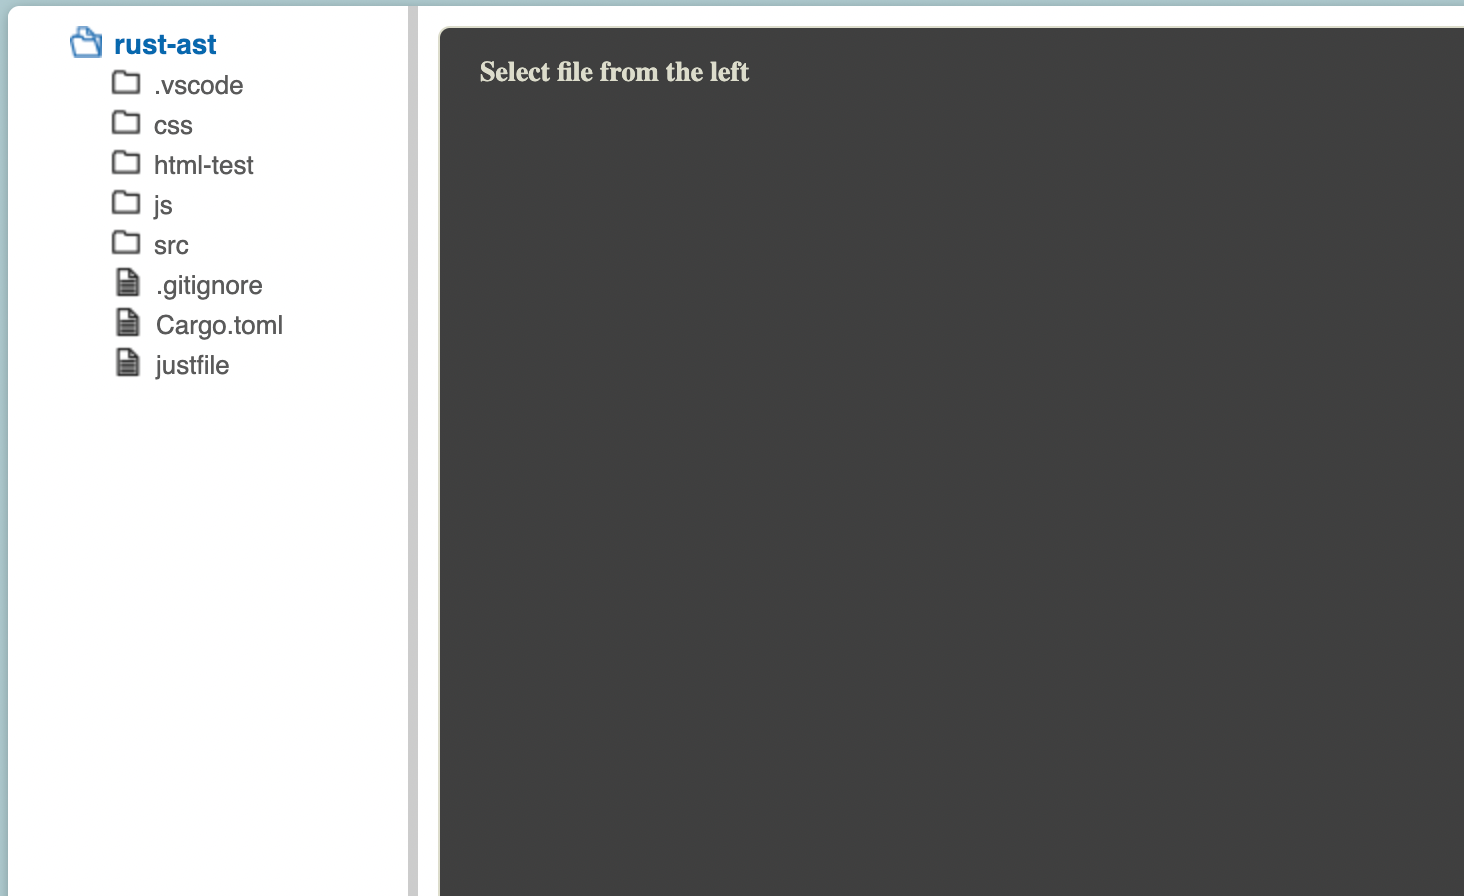
\includegraphics[width=15cm]{figs/screenshots/initial.png}
\caption{Initial content of the report.}
\label{fig:initial}
\end{figure}


Upon clicking on a file name in the project tree, the top section of the code will display the name of the current file, and the highlighted content of the file will be rendered. When hovering over a variable, function, or expression, the user is presented with additional information such as the final type, function signature, or module information. An example of such hover information can be seen in Fig. \ref{fig:hover}.

\begin{figure}[ht]
\centering
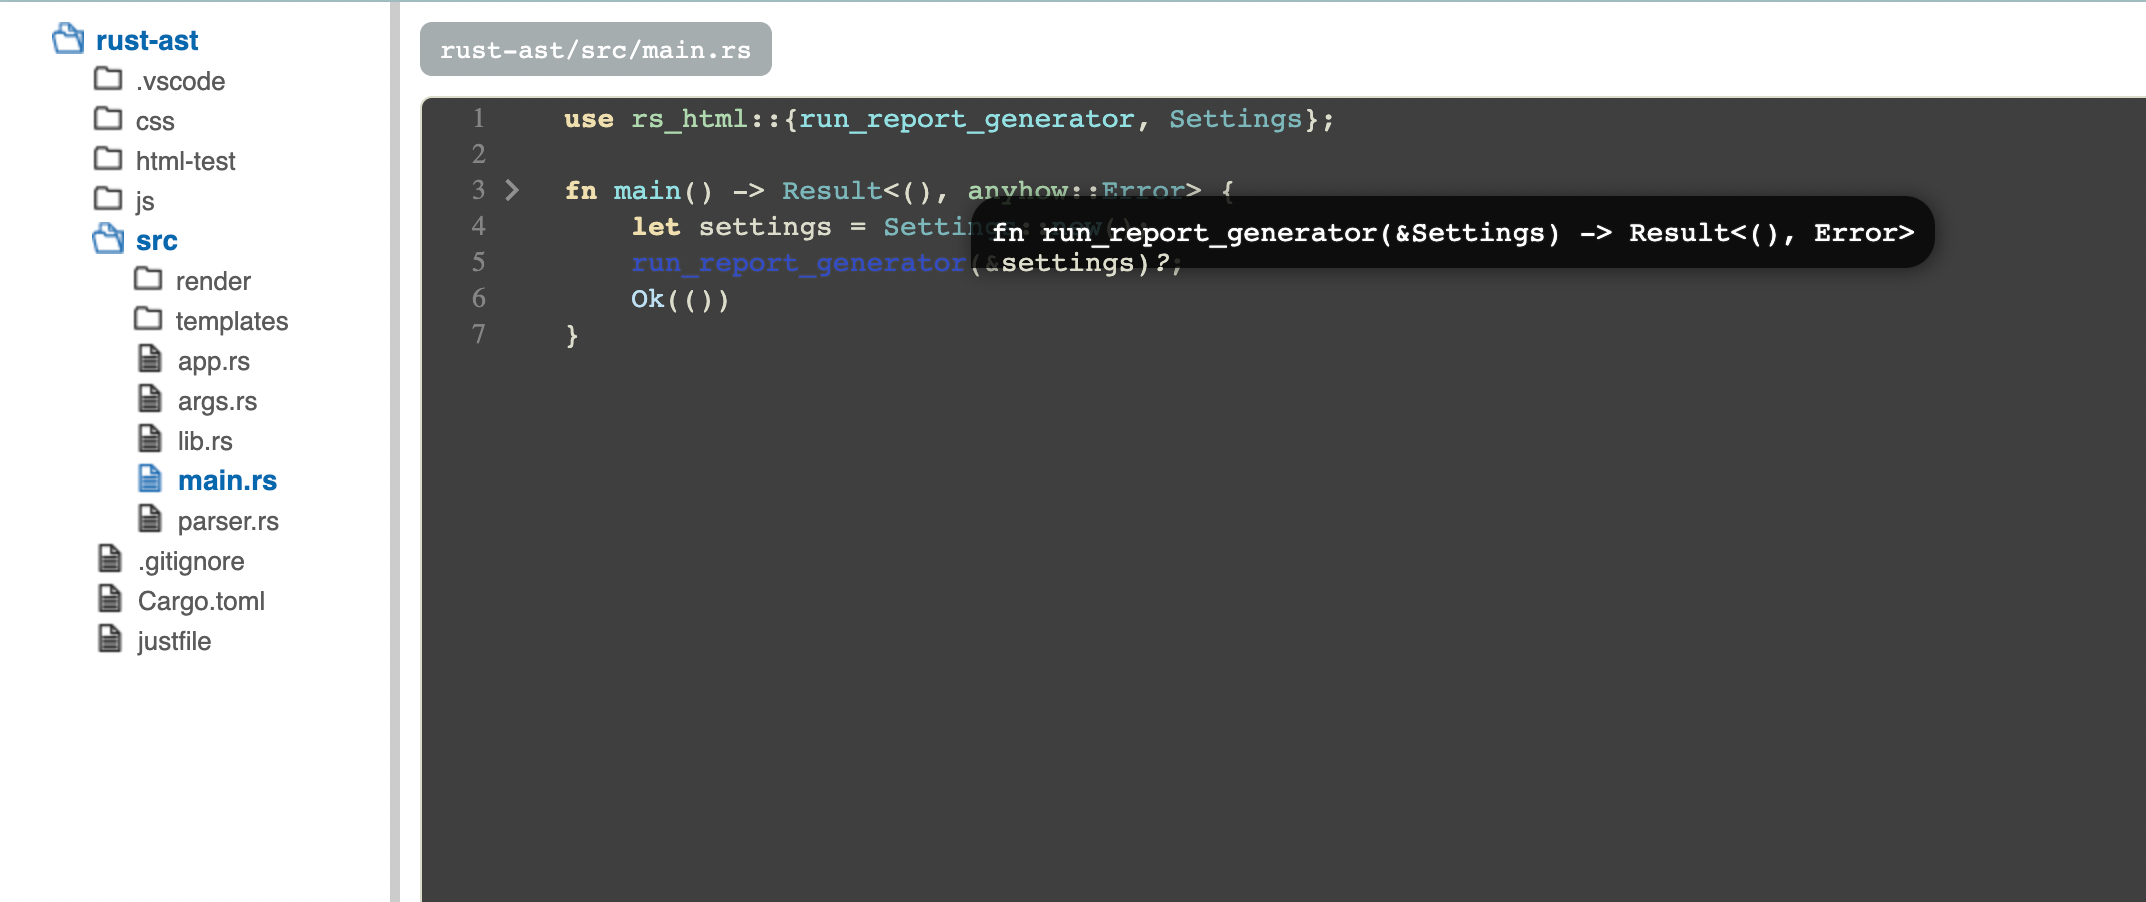
\includegraphics[width=15cm]{figs/screenshots/hover.png}
\caption{Additional information when user cursors token.}
\label{fig:hover}
\end{figure}

When holding down the meta key on the keyboard (\textbf{Cmd} in macOS, \textbf{Ctrl} in Windows and Linux) and clicking on a variable, function, structure, etc., near the clicked location, a navigation menu opens with two tabs. Fig. \ref{fig:nav_def} illustrates the "Definition" tab, which displays the declaration location of the object. Fig. \ref{fig:nav_refs} shows the "References" tab, which lists the places where this object is used. Clicking on a definition or reference location will jump to the desired location, with the necessary line highlighted. As depicted in Fig. \ref{fig:nav_refs}, the yellow background highlights line number 8, serving as a visual indication of the recent jump.

\begin{figure}[ht]
\centering
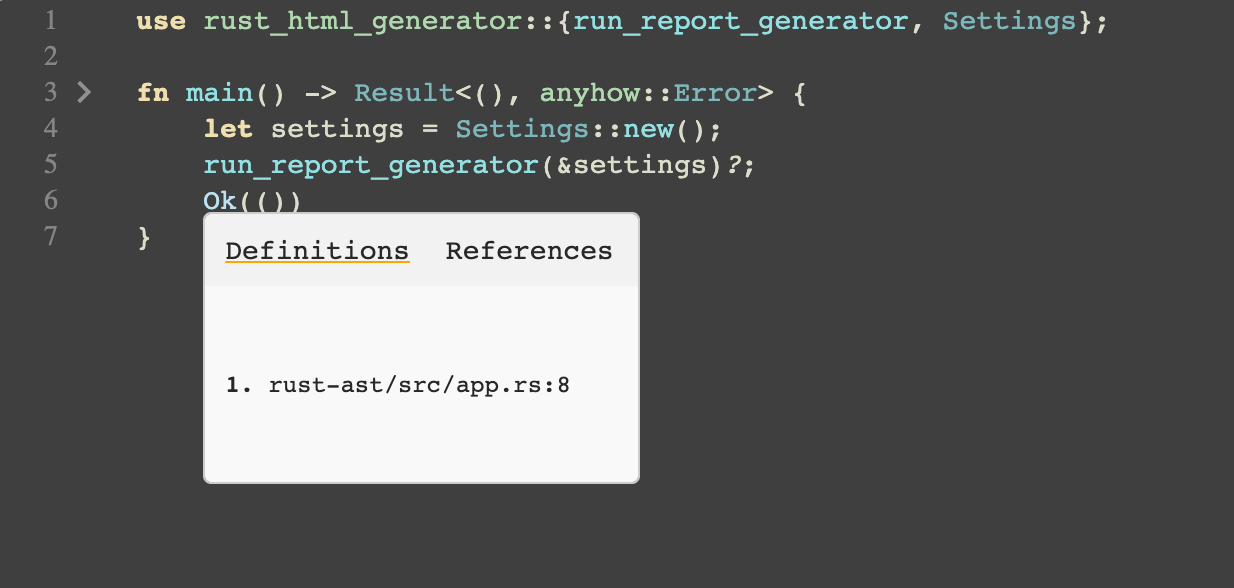
\includegraphics[width=15cm]{figs/screenshots/nav_def_2.png}
\caption{Navigation menu. Definition section.}
\label{fig:nav_def}
\end{figure}


\begin{figure}[ht]
\centering
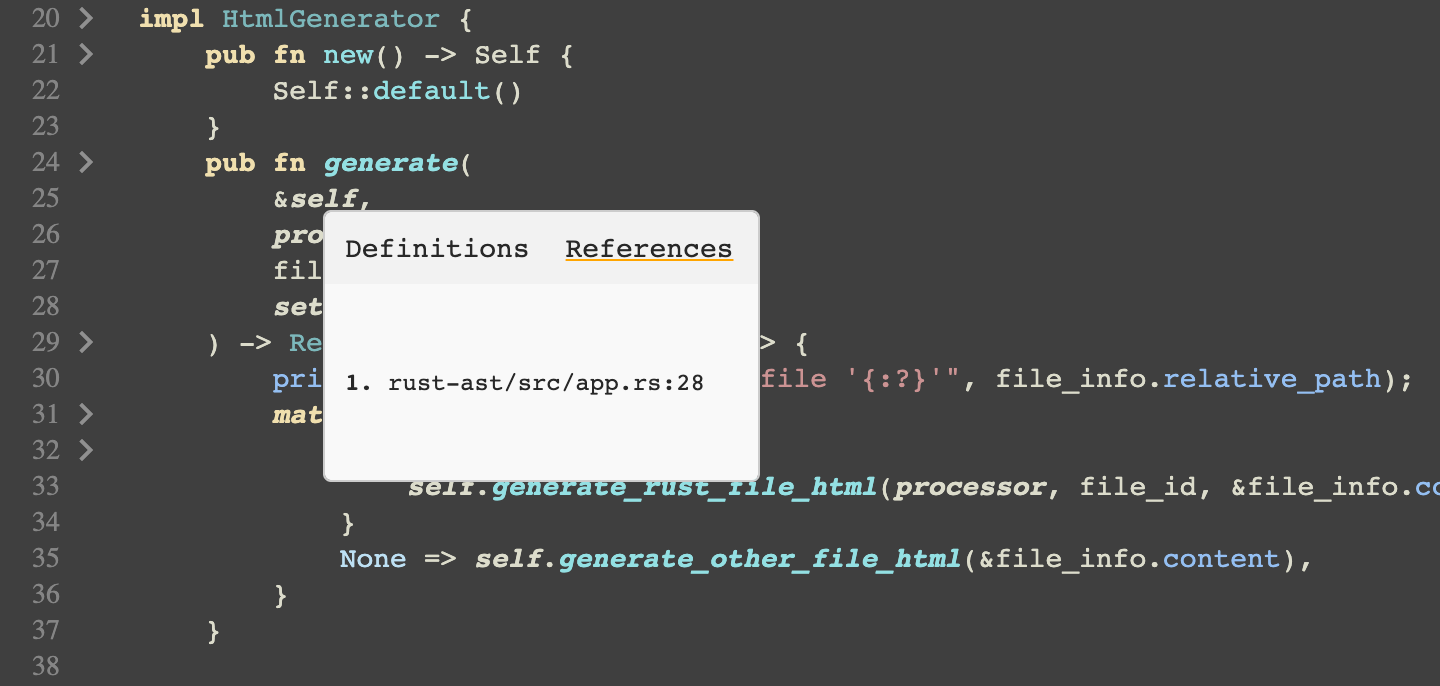
\includegraphics[width=15cm]{figs/screenshots/nav_refs_2.png}
\caption{Navigation menu. References section.}
\label{fig:nav_refs}
\end{figure}

Another beneficial aspect of a report is the ability to collapse or fold lines. This functionality is evident in Fig. \ref{fig:fold}, where each foldable line is accompanied by a right-facing arrow that can be clicked. When pressed, the arrow collapses the lines associated with the corresponding block, including function definitions, function signatures, if statements, match statements, and similar elements.

\begin{figure}[ht]
\centering
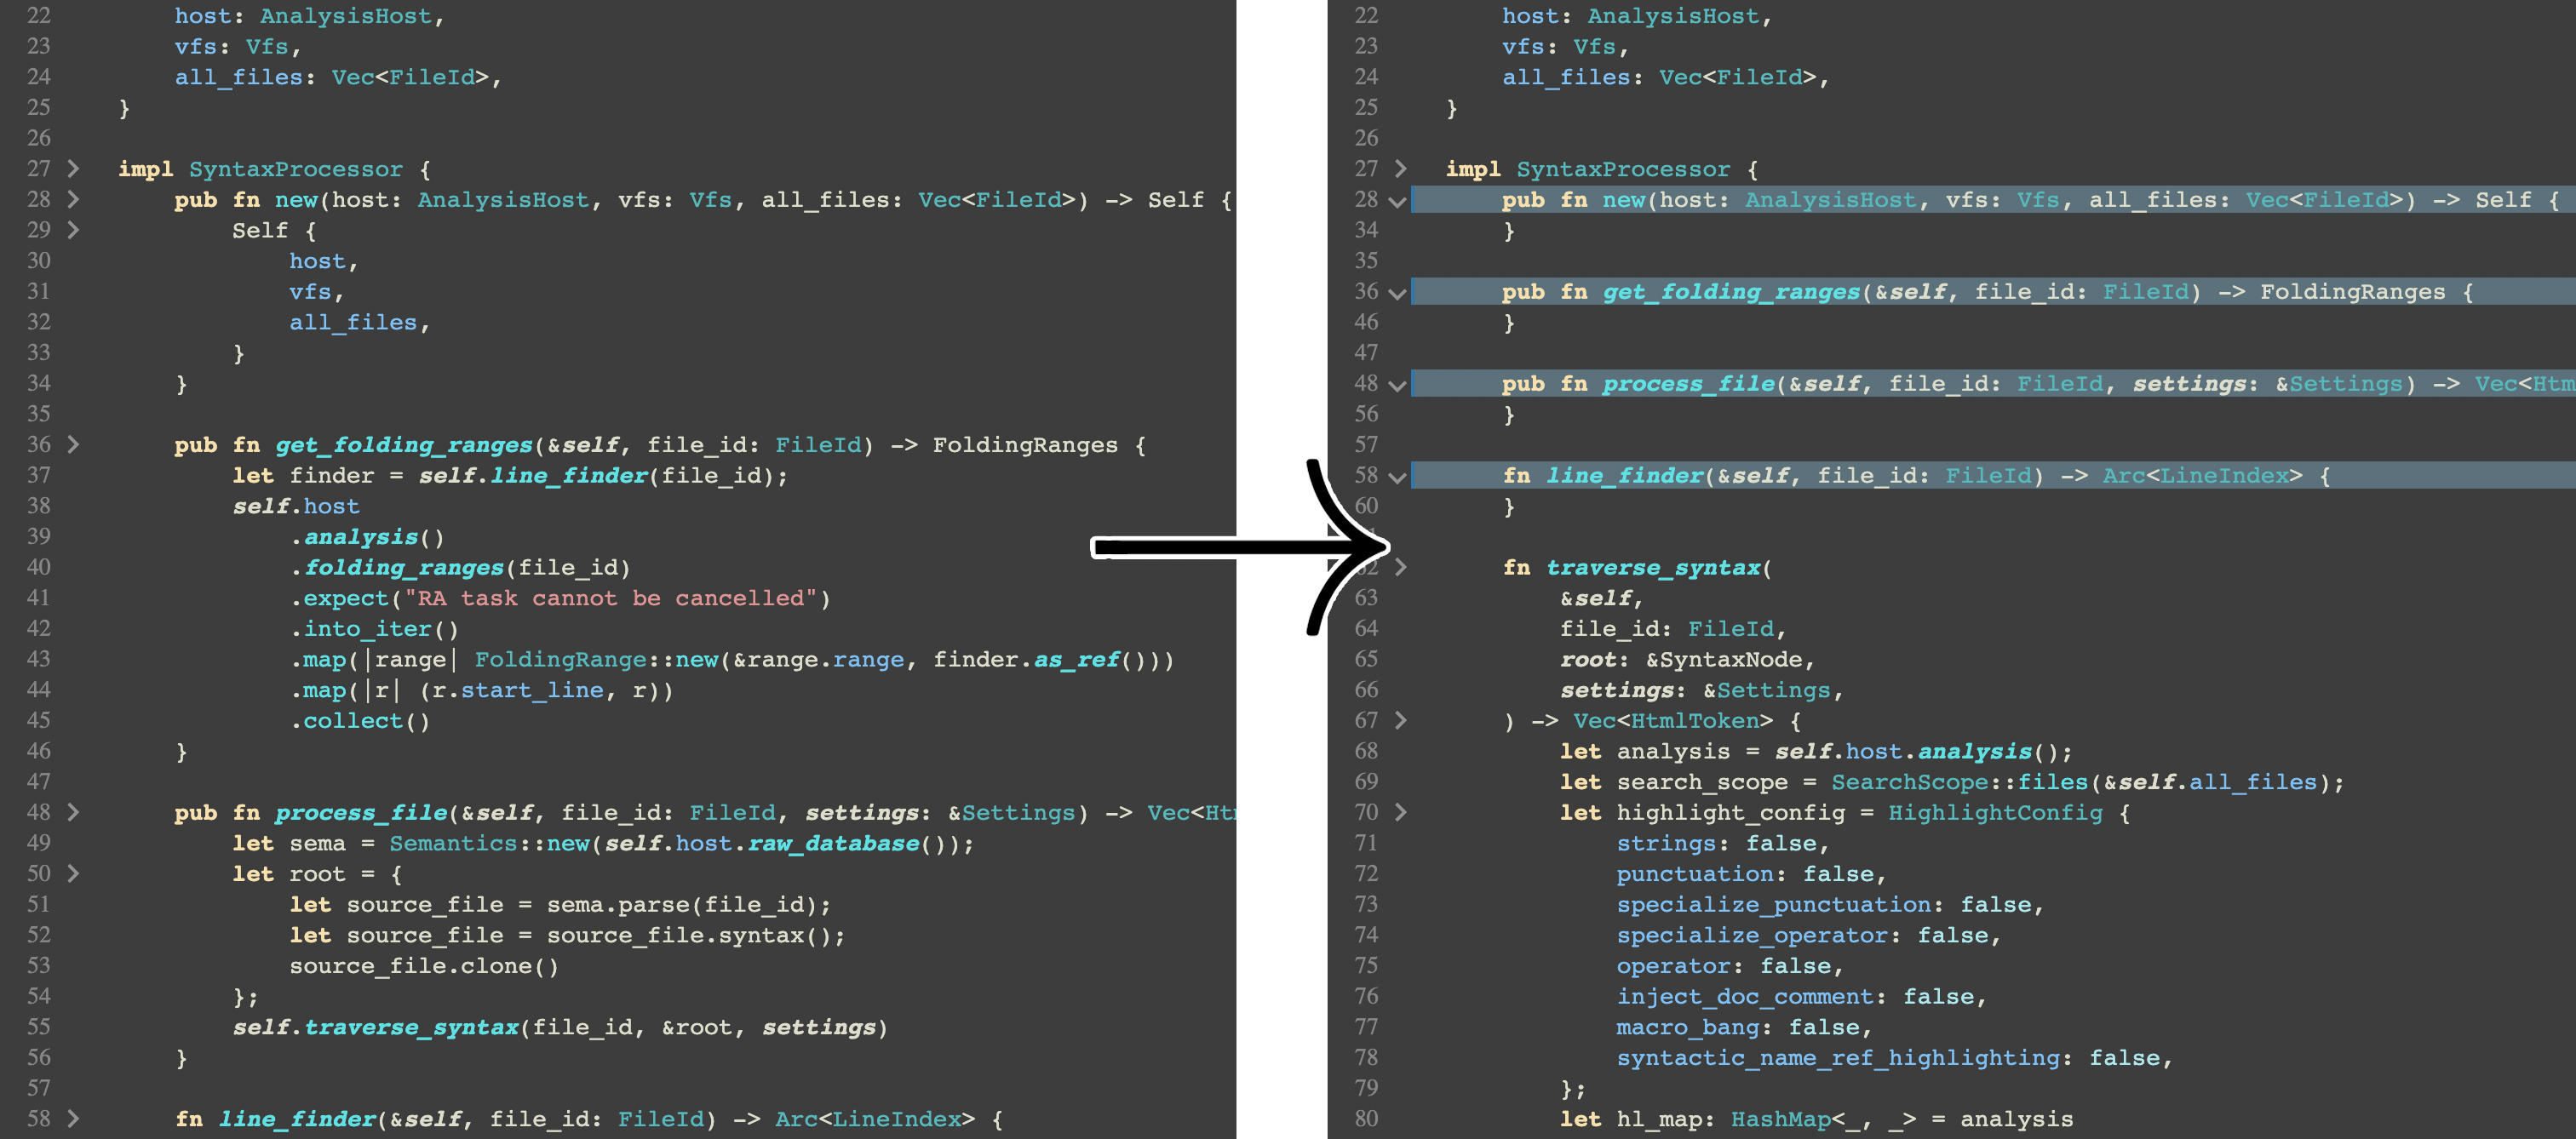
\includegraphics[width=15cm]{figs/screenshots/fold.png}
\caption{Collapsing (folding) code blocks.}
\label{fig:fold}
\end{figure}

\section{Future Work}

We have successfully accomplished our initial objectives and produced a fully operational system. Nevertheless, there exist numerous prospects for future endeavors and enhancements, which are as follows:

\begin{enumerate}
\item \textbf{Customizable Style Themes:} The incorporation of customizable style themes into the system would empower users to personalize the visual representation of Rust code within the HTML report. By introducing this feature, we would augment the overall user experience and cater to the individual preferences and requirements of users.

\item \textbf{Project Search:} The implementation of a project search functionality within the HTML report would furnish users with the ability to swiftly locate specific code snippets, functions, or variables. This notable addition would significantly ameliorate the navigability and accessibility of large-scale projects.

\item \textbf{Synchronization Problem:} Upon the completion of the report, it ceases to remain synchronized with the latest version of the project, as it incorporates the content of all files for the sake of portability. In order to address this issue, we propose the inclusion of an optional button that enables the synchronization of the current project version using a remote git repository.
\end{enumerate}


%% REFERENCES
\printbibliography[heading=bibintoc,title={Bibliography cited}]
% \appendix
\chapter{Extra Stuff}
\blindtext

\chapter{Even More Extra Stuff}
\blindtext
\end{document}

